\documentclass[tikz,border=4pt]{standalone}
\usepackage{tikz}
\usetikzlibrary{arrows.meta,positioning,calc}
\definecolor{cState}{HTML}{DBEAFE}
\definecolor{cBase}{HTML}{E5E7EB}
\definecolor{cTeacher}{HTML}{FCE7F3}
\definecolor{cDelta}{HTML}{FDE68A}
\definecolor{cModel}{HTML}{D1FAE5}
\definecolor{cRecover}{HTML}{CFFAFE}

\begin{document}
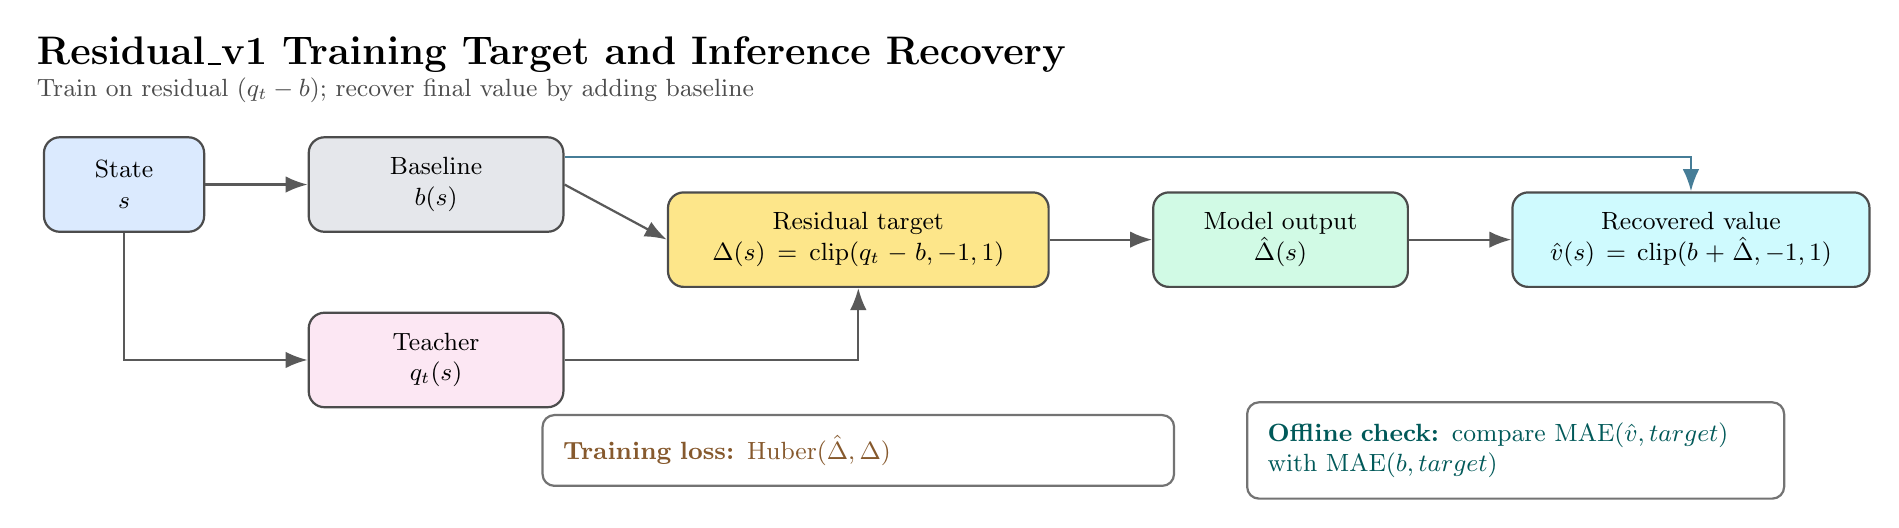
\begin{tikzpicture}[
    font=\small,
    node distance=10mm and 13mm,
    box/.style={draw=black!70, rounded corners=2mm, thick, align=center, minimum height=12mm},
    arr/.style={-{Latex[length=2.8mm]}, thick, draw=black!65},
    note/.style={draw=black!55, rounded corners=1.5mm, thick, align=left, fill=white, text width=75mm, inner sep=2.6mm}
]
\node[draw=none, font=\Large\bfseries, anchor=west] at (-0.2,4.0) {Residual\_v1 Training Target and Inference Recovery};
\node[draw=none, font=\small, text=black!70, anchor=west] at (-0.2,3.55) {Train on residual $(q_t-b)$; recover final value by adding baseline};

\node[box, fill=cState, text width=18mm, anchor=west] (s) at (0,2.35) {State\\$s$};
\node[box, fill=cBase, text width=30mm, right=of s] (b) {Baseline\\$b(s)$};
\node[box, fill=cTeacher, text width=30mm, below=of b] (qt) {Teacher\\$q_t(s)$};
\node[box, fill=cDelta, text width=46mm, right=of b, yshift=-7mm] (delta) {Residual target\\$\Delta(s)=\mathrm{clip}(q_t-b,-1,1)$};
\node[box, fill=cModel, text width=30mm, right=of delta] (dhat) {Model output\\$\hat{\Delta}(s)$};
\node[box, fill=cRecover, text width=43mm, right=of dhat] (vhat) {Recovered value\\$\hat{v}(s)=\mathrm{clip}(b+\hat{\Delta},-1,1)$};

\draw[arr] (s) -- (b);
\draw[arr] (s) |- (qt.west);
\draw[arr] (b.east) -- (delta.west);
\draw[arr] (qt.east) -| (delta.south);
\draw[arr] (delta.east) -- (dhat.west);
\draw[arr] (dhat.east) -- (vhat.west);
\coordinate (b2v_start) at ([yshift=3.5mm]b.east);
\coordinate (b2v_turn) at (b2v_start -| vhat.north);
\draw[arr, draw=cyan!55!black] (b2v_start) -- (b2v_turn) -- ([yshift=3mm]vhat.north) -- (vhat.north);

\node[note, below=16mm of delta, text=brown!70!black] (loss) {\textbf{Training loss:} $\mathrm{Huber}(\hat{\Delta},\Delta)$};
\node[note, right=9mm of loss, text=teal!70!black, text width=63mm] (offline) {\textbf{Offline check:} compare $\mathrm{MAE}(\hat{v},target)$ with $\mathrm{MAE}(b,target)$};

\end{tikzpicture}
\end{document}
